Para as obtenção das medidas desejadas foi empregado um laser de luz verde aproximadamente monocromática ($\lambda = \SI{532}{\nano\meter}$). 

Inicialmente, foi feito o alinhamento do laser, de forma que as medições pudessem ser realizadas com precisão. Para tal, um vidro (figura \ref{fig:rede}) contendo diversas fendas variadas, impressas por litografia em um vidro metálico, foi alinhado perpendicularmente ao feixe do laser. Em seguida o feixe foi alinhado com trilho em que o vidro com as fendas estava montado, completando a fase de alinhamento do experimento. 

\begin{figure}[H]
	\centering	    
	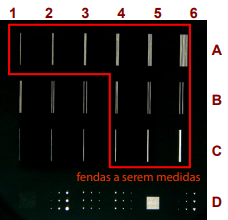
\includegraphics[scale=0.6]{figuras/rede_dif.png}
	\caption{Vidro e fendas utilizadas}
	\label{fig:rede}
\end{figure}

A fim de coletar os dados, buscando medir padrões de difração para fendas simples, o laser foi incidido na fenda C4, de forma que o padrão de difração pudesse ser observado em um papel milimetrado de $5x5\si{\milli\meter}$ utilizado como anteparo, posicionado a \SI{184,5}{\centi\meter}. O procedimento foi repetido para as fendas C5 e C6.

Na sequência, foram medidos os padrões para fendas duplas e múltiplas. o mesmo procedimento anterior foi feito utilizando as fenda B4,B5 e B6 e A1 até A6, respectivamente.